% Layer-frequency distribution of CacheJPEG DCT coefficients.
\begin{figure}[t]
  \centering
  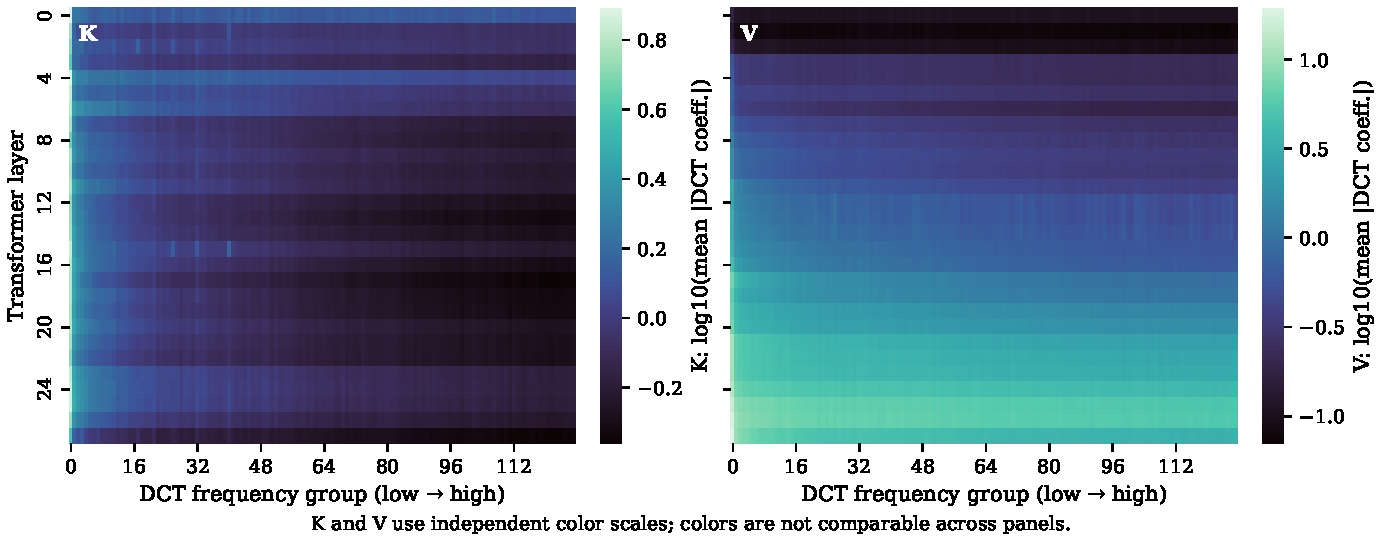
\includegraphics[width=0.95\textwidth]{tmp/dct_layer_frequency_heatmap.pdf}
  \caption{Layer-wise frequency distribution of K/V DCT coefficients. Color denotes the base-10 logarithm of mean absolute coefficient magnitude. K and V use independent color scales to expose their internal frequency patterns; colors are not directly comparable across panels.}
  \label{fig:dct-layer-frequency}
\end{figure}

% Frequency-dimension structure at representative layers.
\begin{figure}[t]
  \centering
  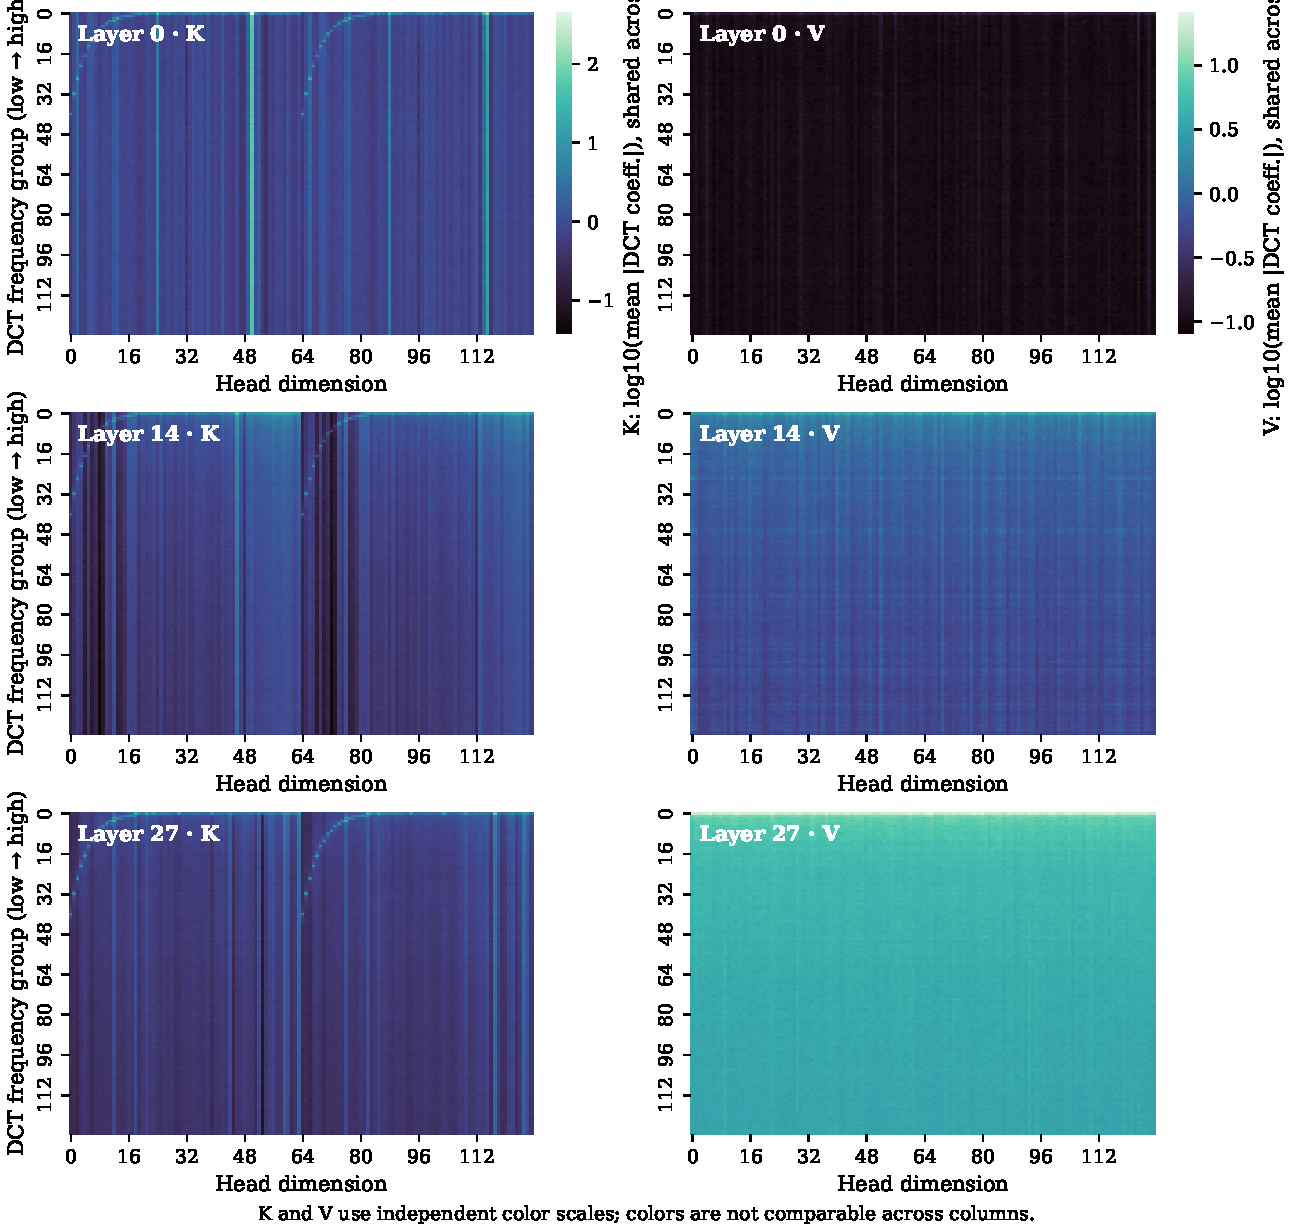
\includegraphics[width=0.95\textwidth]{tmp/dct_frequency_dimension_heatmap.pdf}
  \caption{Frequency-by-head-dimension heatmaps of K/V DCT coefficients at representative transformer layers. Each component uses a color scale shared across all displayed layers, while K and V retain independent scales.}
  \label{fig:dct-frequency-dimension}
\end{figure}
